\subsection{Messergebnisse und Auswertung}
Die Fehler der Counts $N$ sind poissonverteilt und betragen demnach $s_N = \sqrt{N}$. Sie sind in den Graphen der Spektren nicht eingezeichnet, 
da dies zu unübersichtlich ist. Bei den Fits der einzelnen Peaks sind die Fehler eingezeichnet, um die Übereinstimmung der gemessenen Werte 
mit dem theoretischen Modell zu visualisieren.
\subsubsection{CdTe-Detektor}
\paragraph{Spektren}
Die Spektren von \co und \am sind in \autoref{img:cdte:co:spektrum} und \autoref{img:cdte:am:spektrum} dargestellt. Man erkennt den 59.5\,keV-Peak 
von \am\, bei Kanal 300, den 122.06\,keV-Peak von \co\, bei Kanal 600 und den 136.47\,keV-Peak von \co\, bei Kanal 700.
\begin{figure}[H]
\begin{center}
  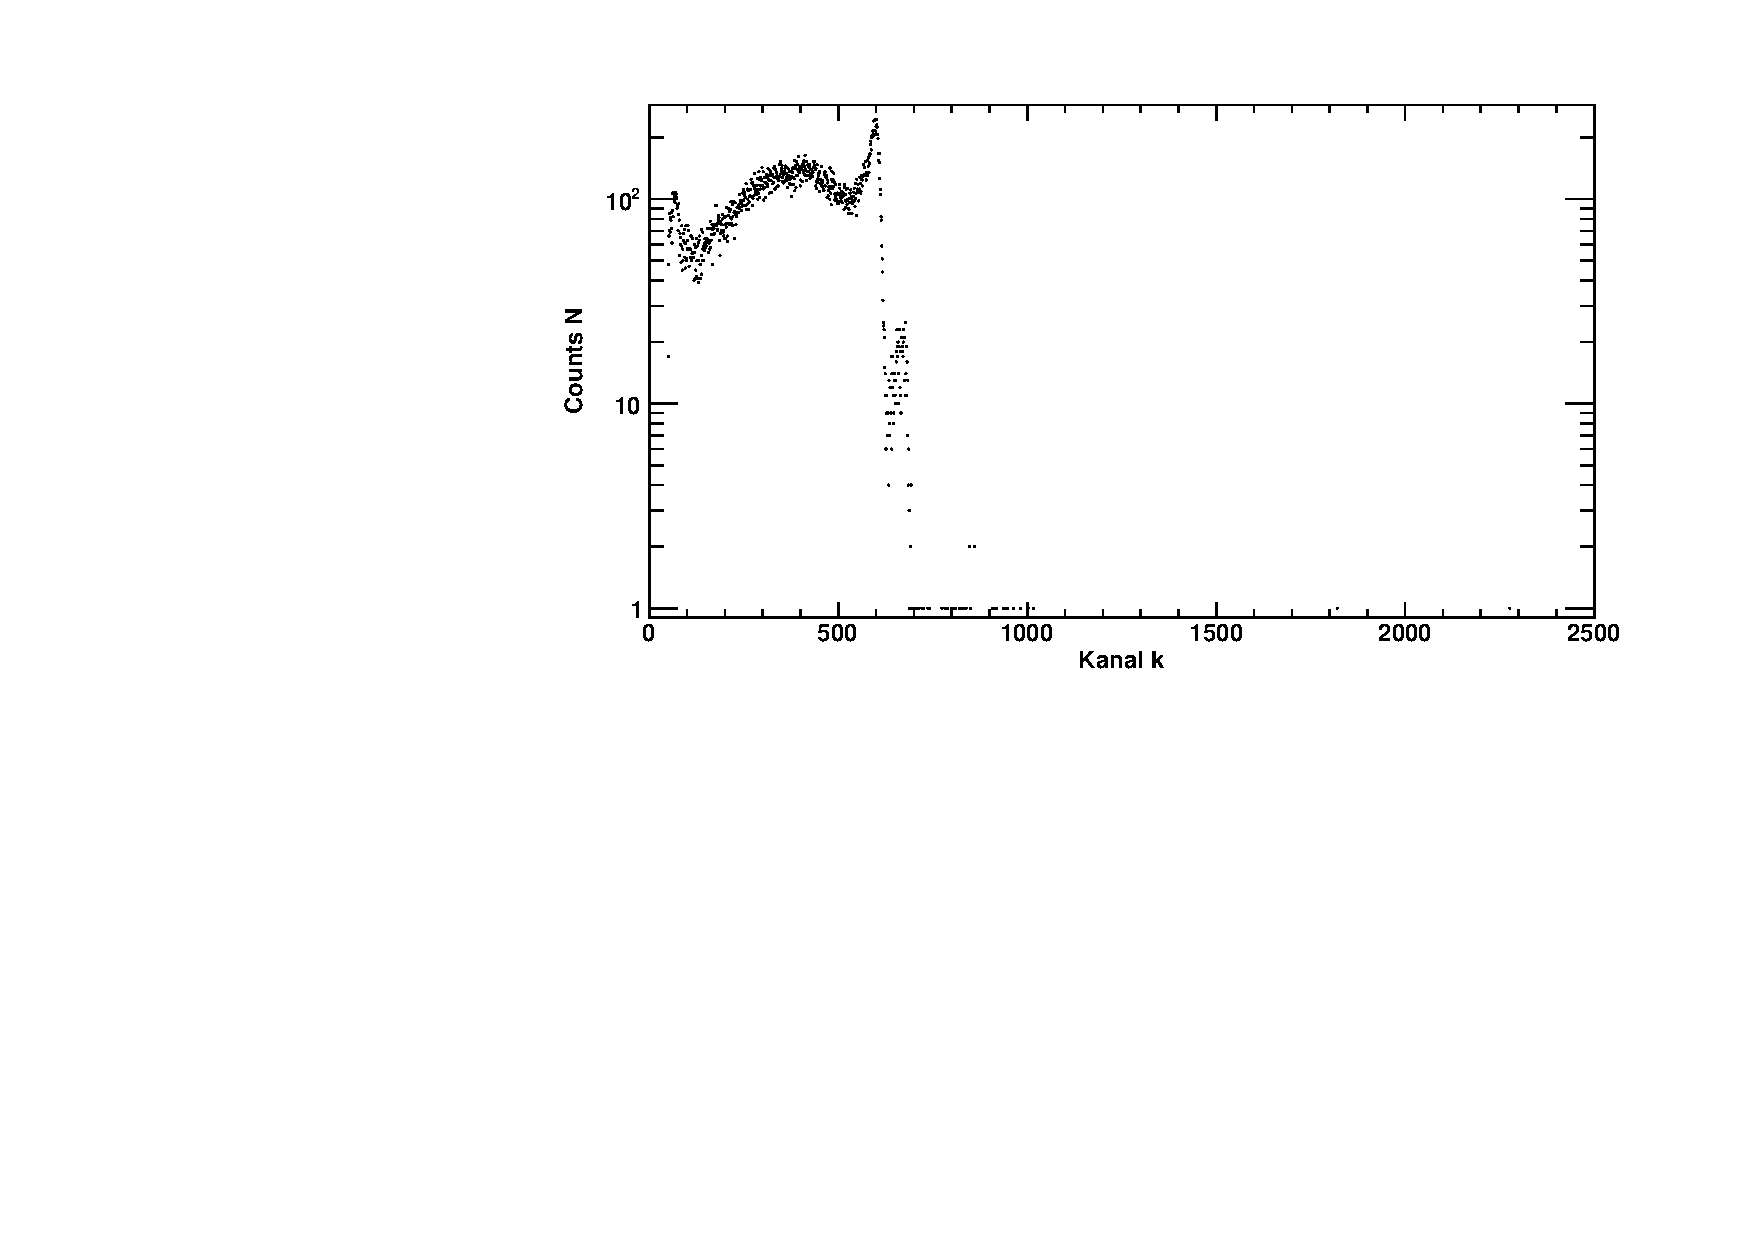
\includegraphics[width=\textwidth]{../img/part3/Co-CdTe_spectrum.pdf}
  \caption{Spektrum von \co, gemessen mit dem CdTe-Detektor.}
  \label{img:cdte:co:spektrum}
\end{center}
\end{figure}

\begin{figure}[H]
\begin{center}
  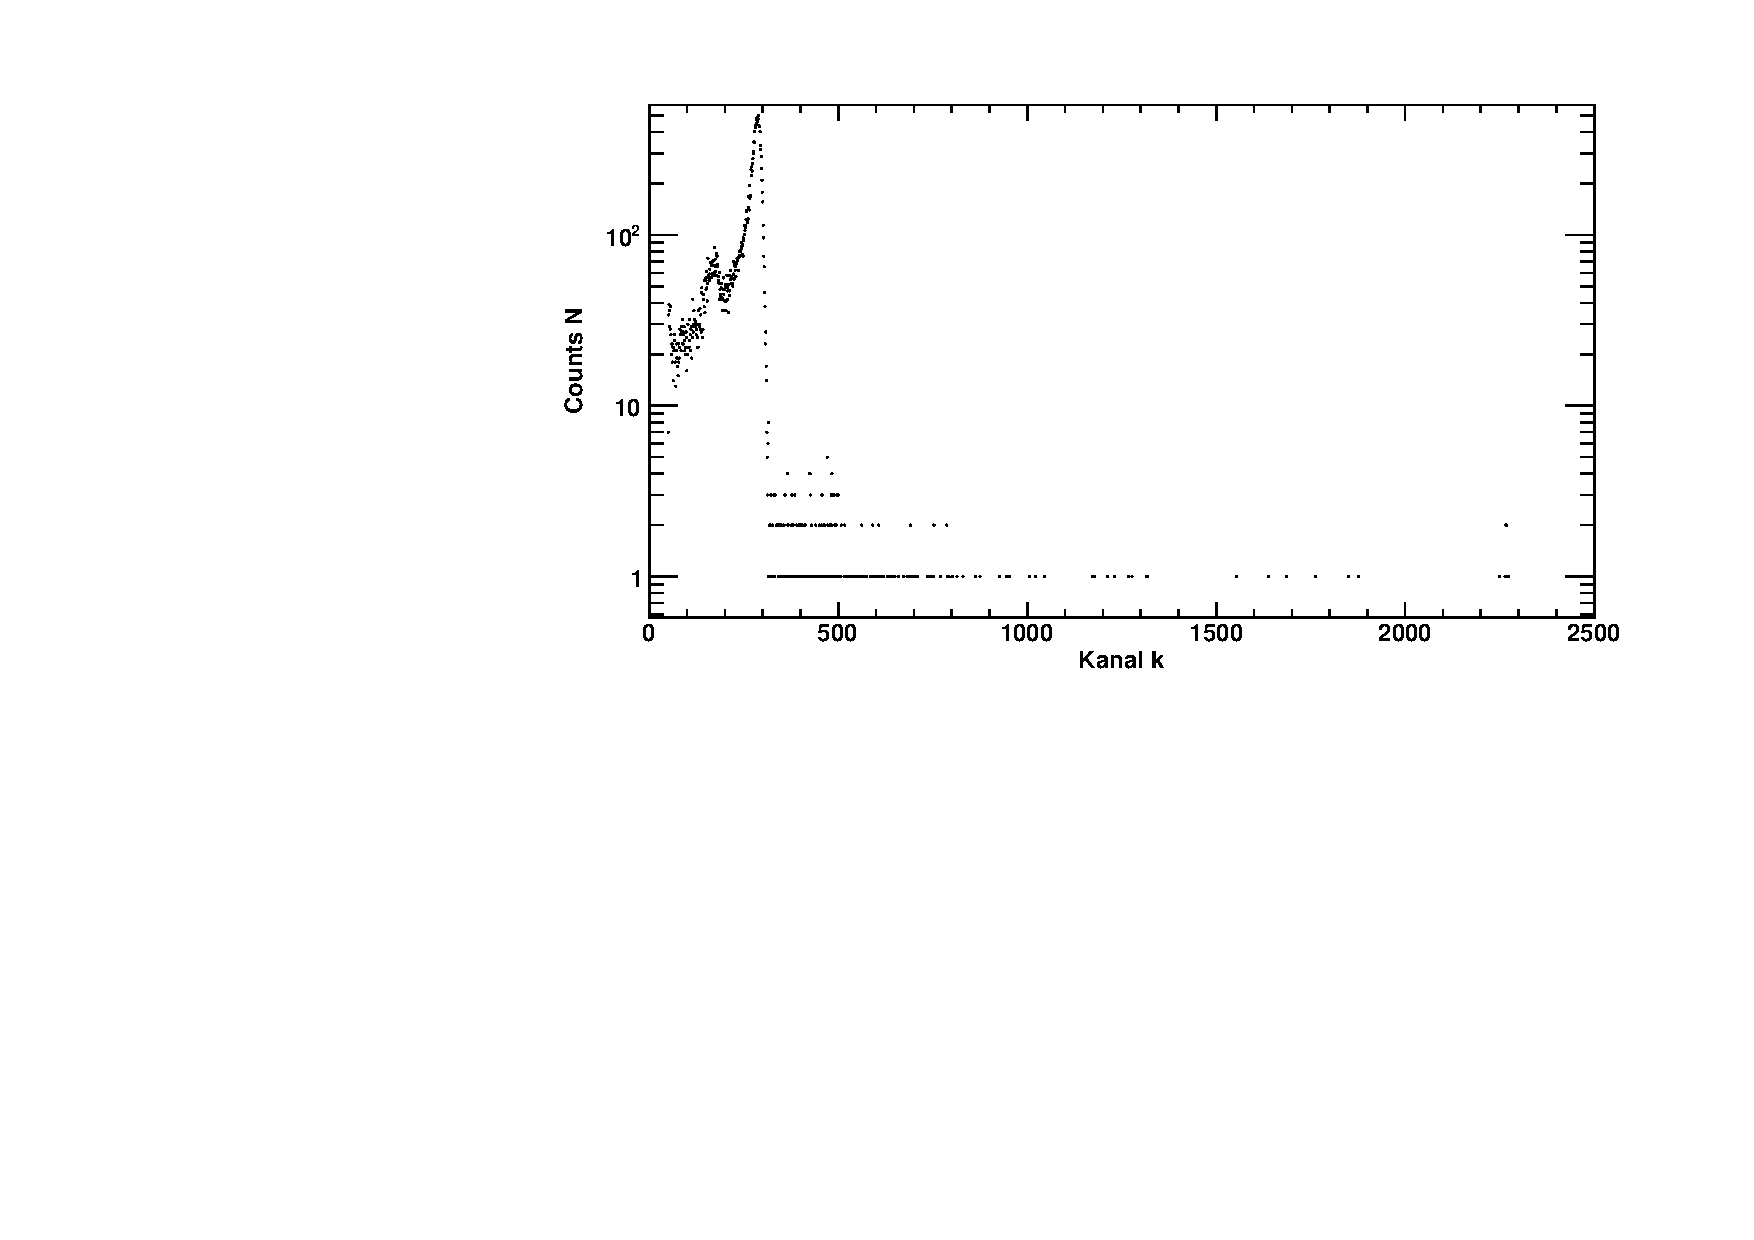
\includegraphics[width=\textwidth]{../img/part3/Am-CdTe_spectrum.pdf}
  \caption{Spektrum von \am, gemessen mit dem CdTe-Detektor.}
  \label{img:cdte:am:spektrum}
\end{center}
\end{figure}


\paragraph{Peaks}
Die einzelnen Peaks werden mit einer normierten Gauß-Kurve gefittet.
\begin{equation}
  \label{eq:part3:normgauss}
  N(k) = A \cdot \frac{1}{\sqrt{2\pi \cdot \sigma^2}} \cdot e^{-\frac{1}{2} \left( \frac{k-k_c}{\sigma} \right)^2}
\end{equation}
Die Fits sind in \autoref{img:am:cdte:peak0}, \autoref{img:co:cdte:peak0} und \autoref{img:co:cdte:peak1} dargestellt. Wie man erkennt, sind die 
Peaks nicht ganz symmetrisch verteilt. %TODO verweis staatsex
\begin{figure}[H]
\begin{center}
  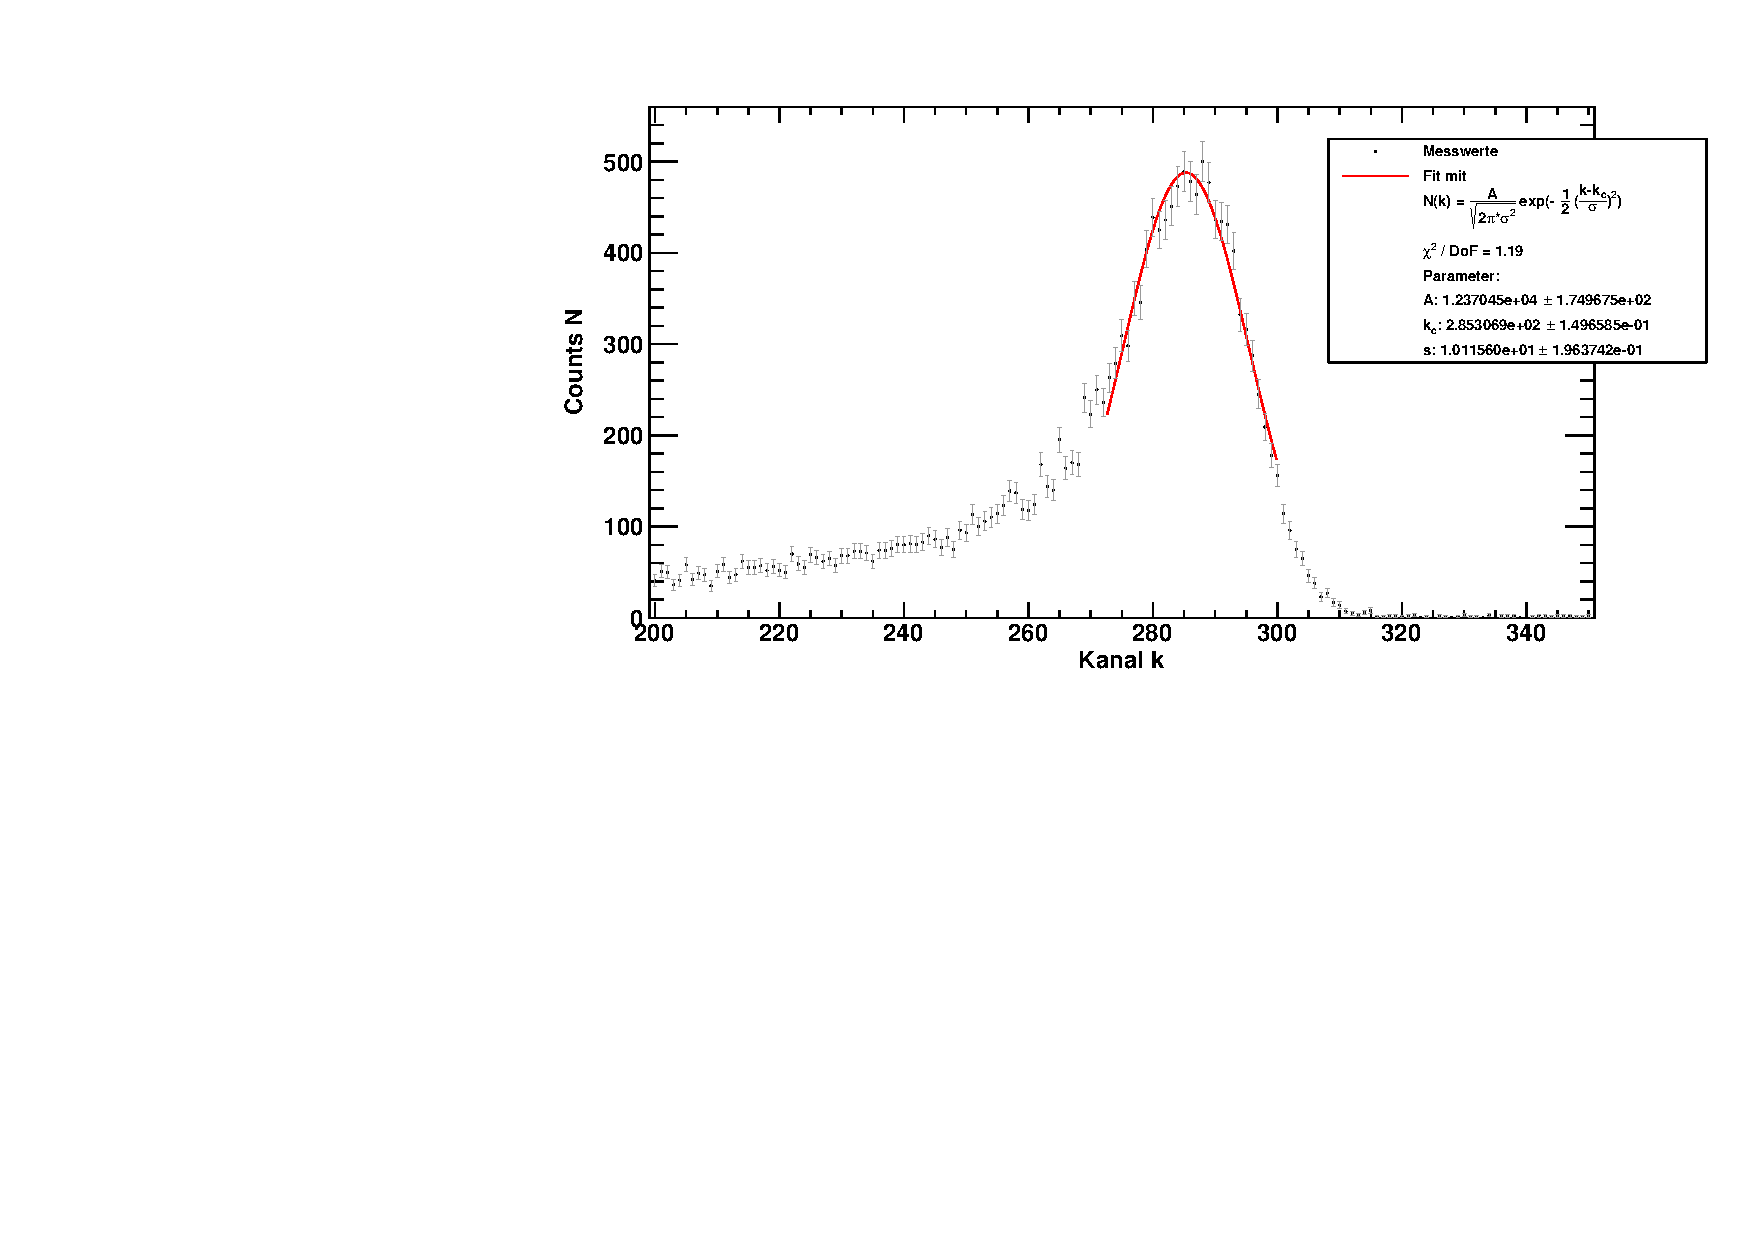
\includegraphics[width=\textwidth]{../img/part3/Am-CdTe_00.pdf}
  \caption{59.5\,keV-Peak von \am, gemessen mit dem CdTe-Detektor.}
  \label{img:am:cdte:peak0}
\end{center}
\end{figure}

\begin{figure}[H]
\begin{center}
  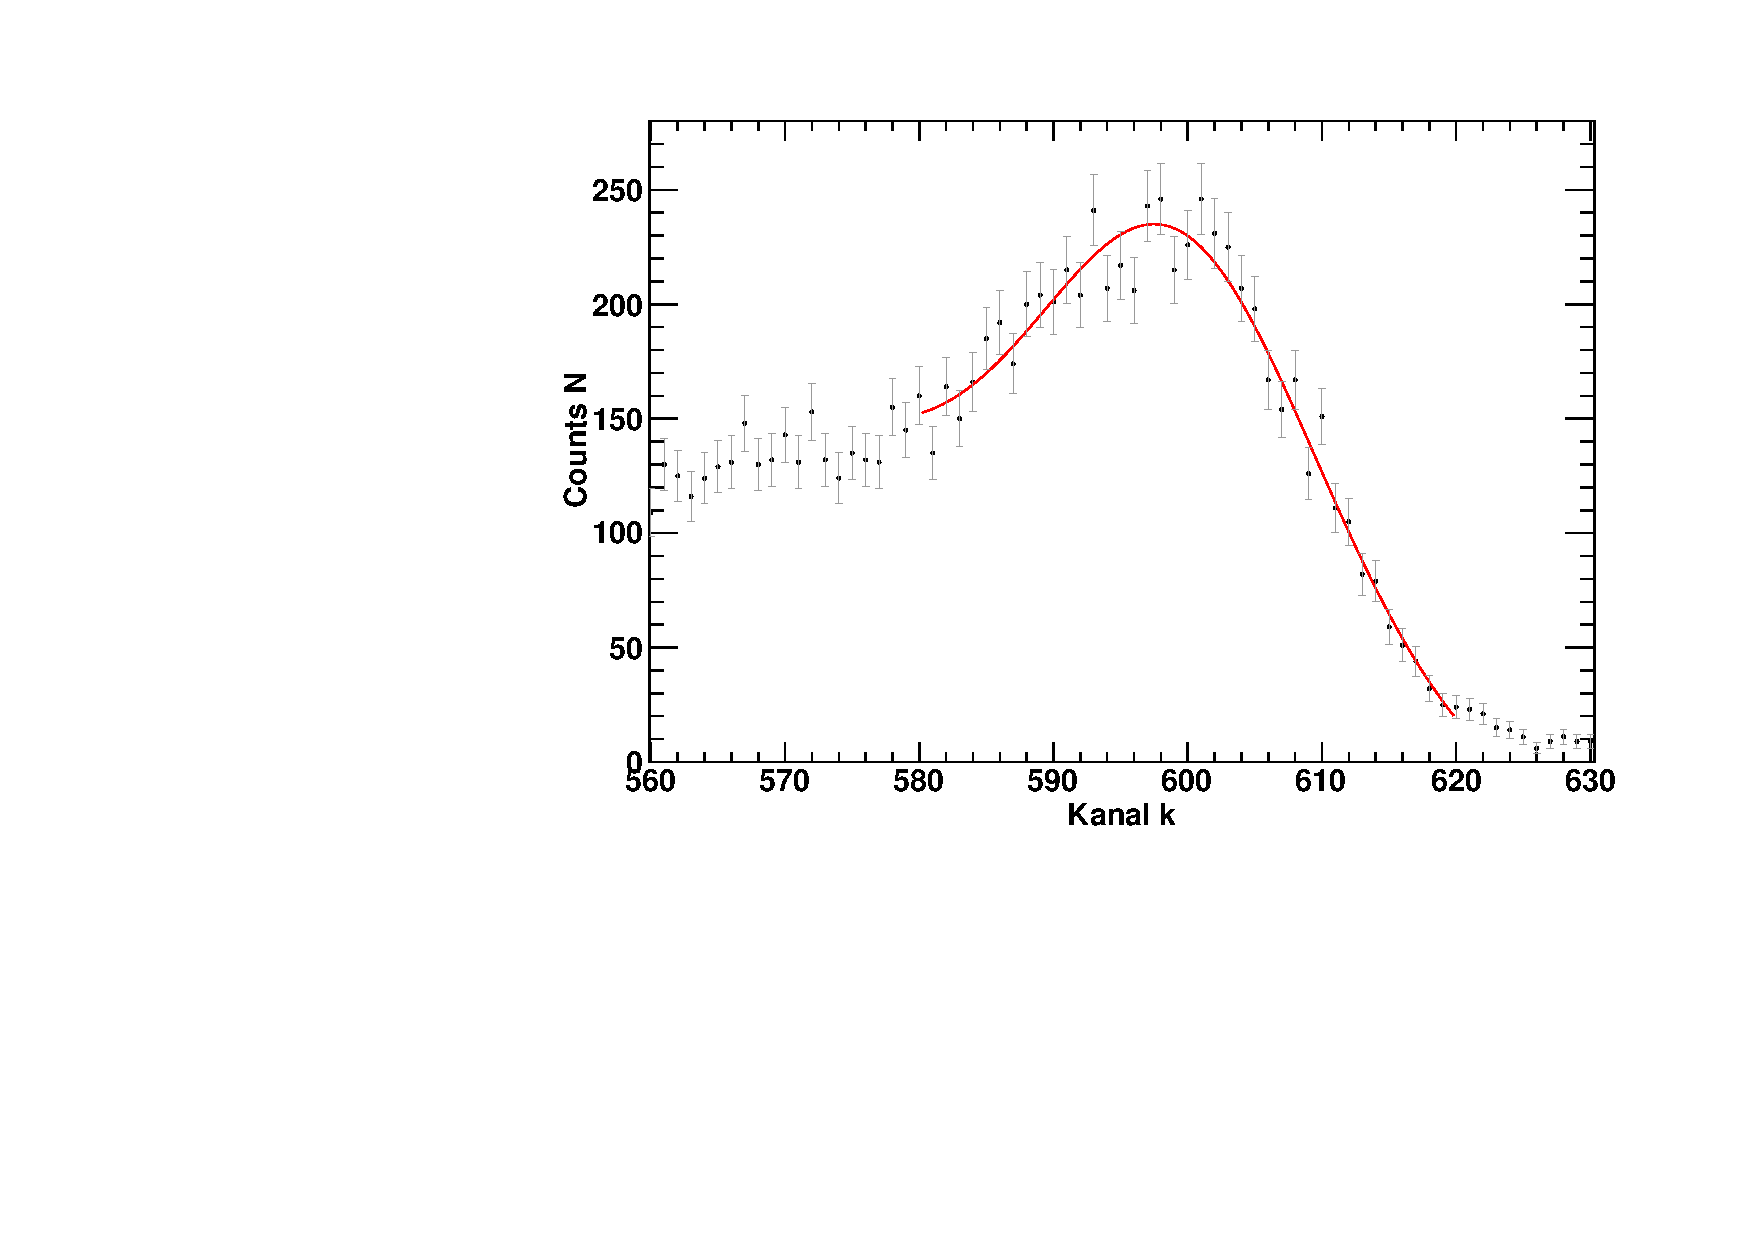
\includegraphics[width=\textwidth]{../img/part3/Co-CdTe_00.pdf}
  \caption{122.06\,keV-Peak von \co, gemessen mit dem CdTe-Detektor.}
  \label{img:co:cdte:peak0}
\end{center}
\end{figure}

\begin{figure}[H]
\begin{center}
  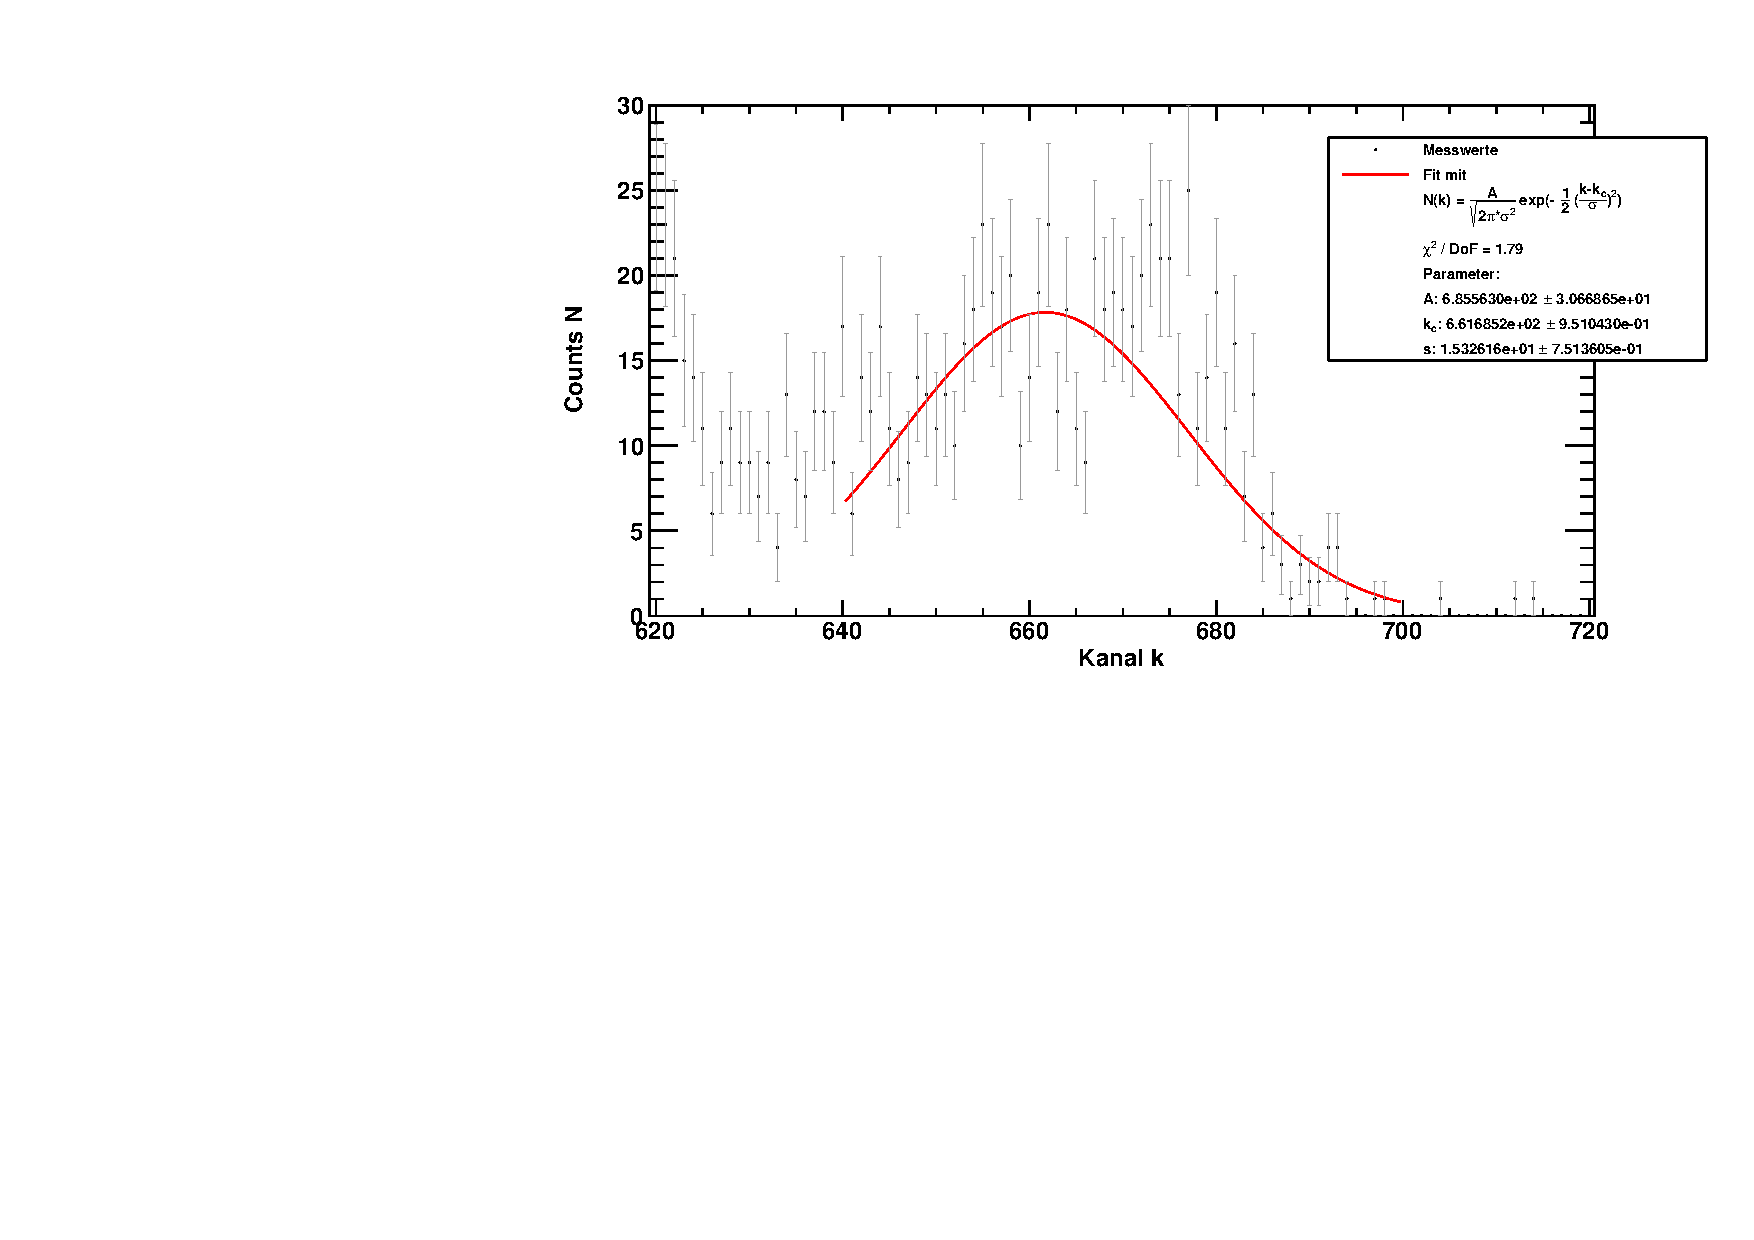
\includegraphics[width=\textwidth]{../img/part3/Co-CdTe_01.pdf}
  \caption{136.47\,keV-Peak von \co, gemessen mit dem CdTe-Detektor.}
  \label{img:co:cdte:peak1}
\end{center}
\end{figure}

\paragraph{Energieeichung}
Platzhalter
\begin{figure}[H]
\begin{center}
  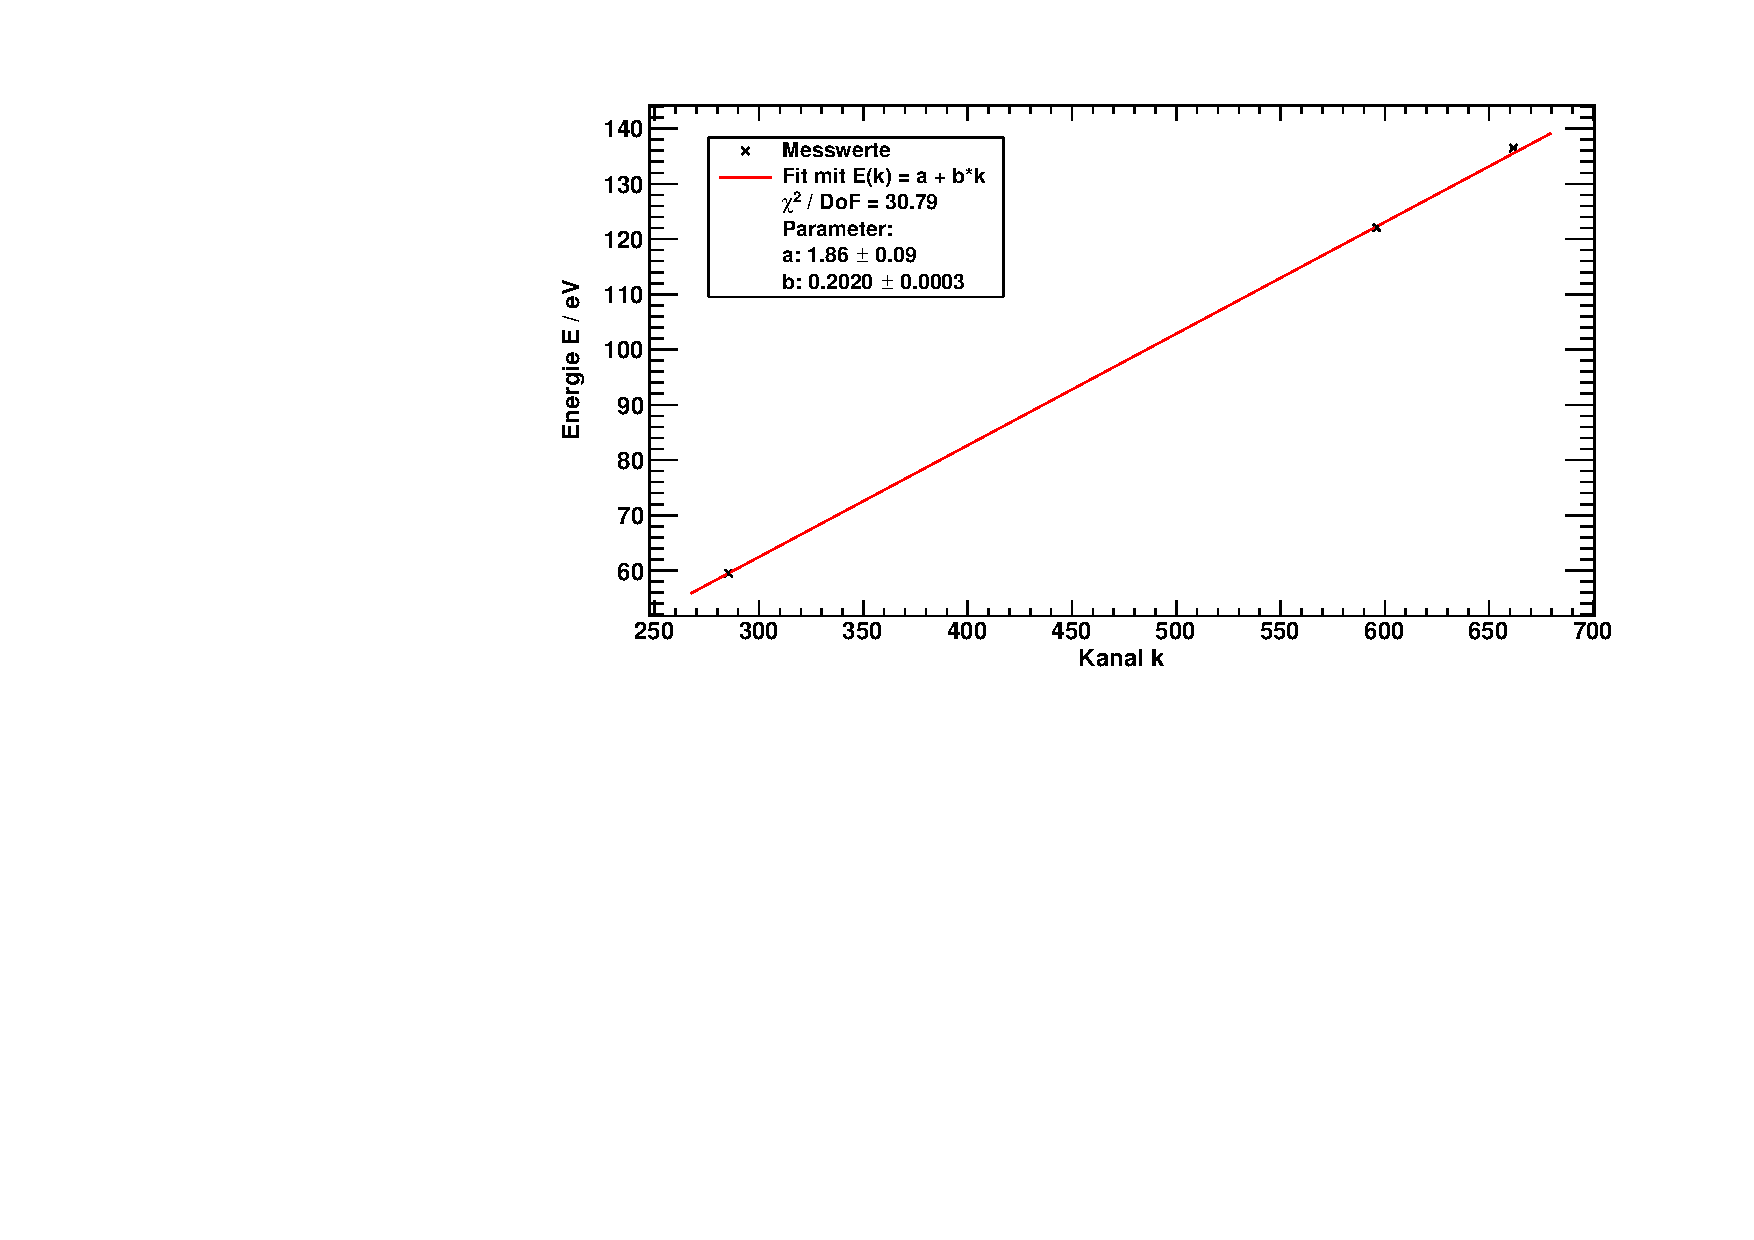
\includegraphics[width=\textwidth]{../img/part3/energygauge_CdTe.pdf}
  \caption{caption}
  \label{img:cdte:energygauge}
\end{center}
\end{figure}

\paragraph{Absorptionswahrscheinlichkeiten}

\paragraph{Relative Energieauflösung}

\subsubsection{Si-Detektor}
\paragraph{Spektren}
In den Spektren von \co und \am (\autoref{img:si:co:spektrum} und \autoref{img:si:am:spektrum}) sieht den 59.5\,keV-Peak 
von \am\, bei Kanal 300 und den 122.06\,keV-Peak von \co\, bei Kanal 600. Der 136.47\,keV-Peak von \co\, lässt sich im Gesamtspektrum 
ohne Vergrößerung (der x-Achse) nicht mehr erkennen, er lässt sich allerdings direkt rechts neben dem 122.06\,keV-Peak finden.
\begin{figure}[H]
\begin{center}
  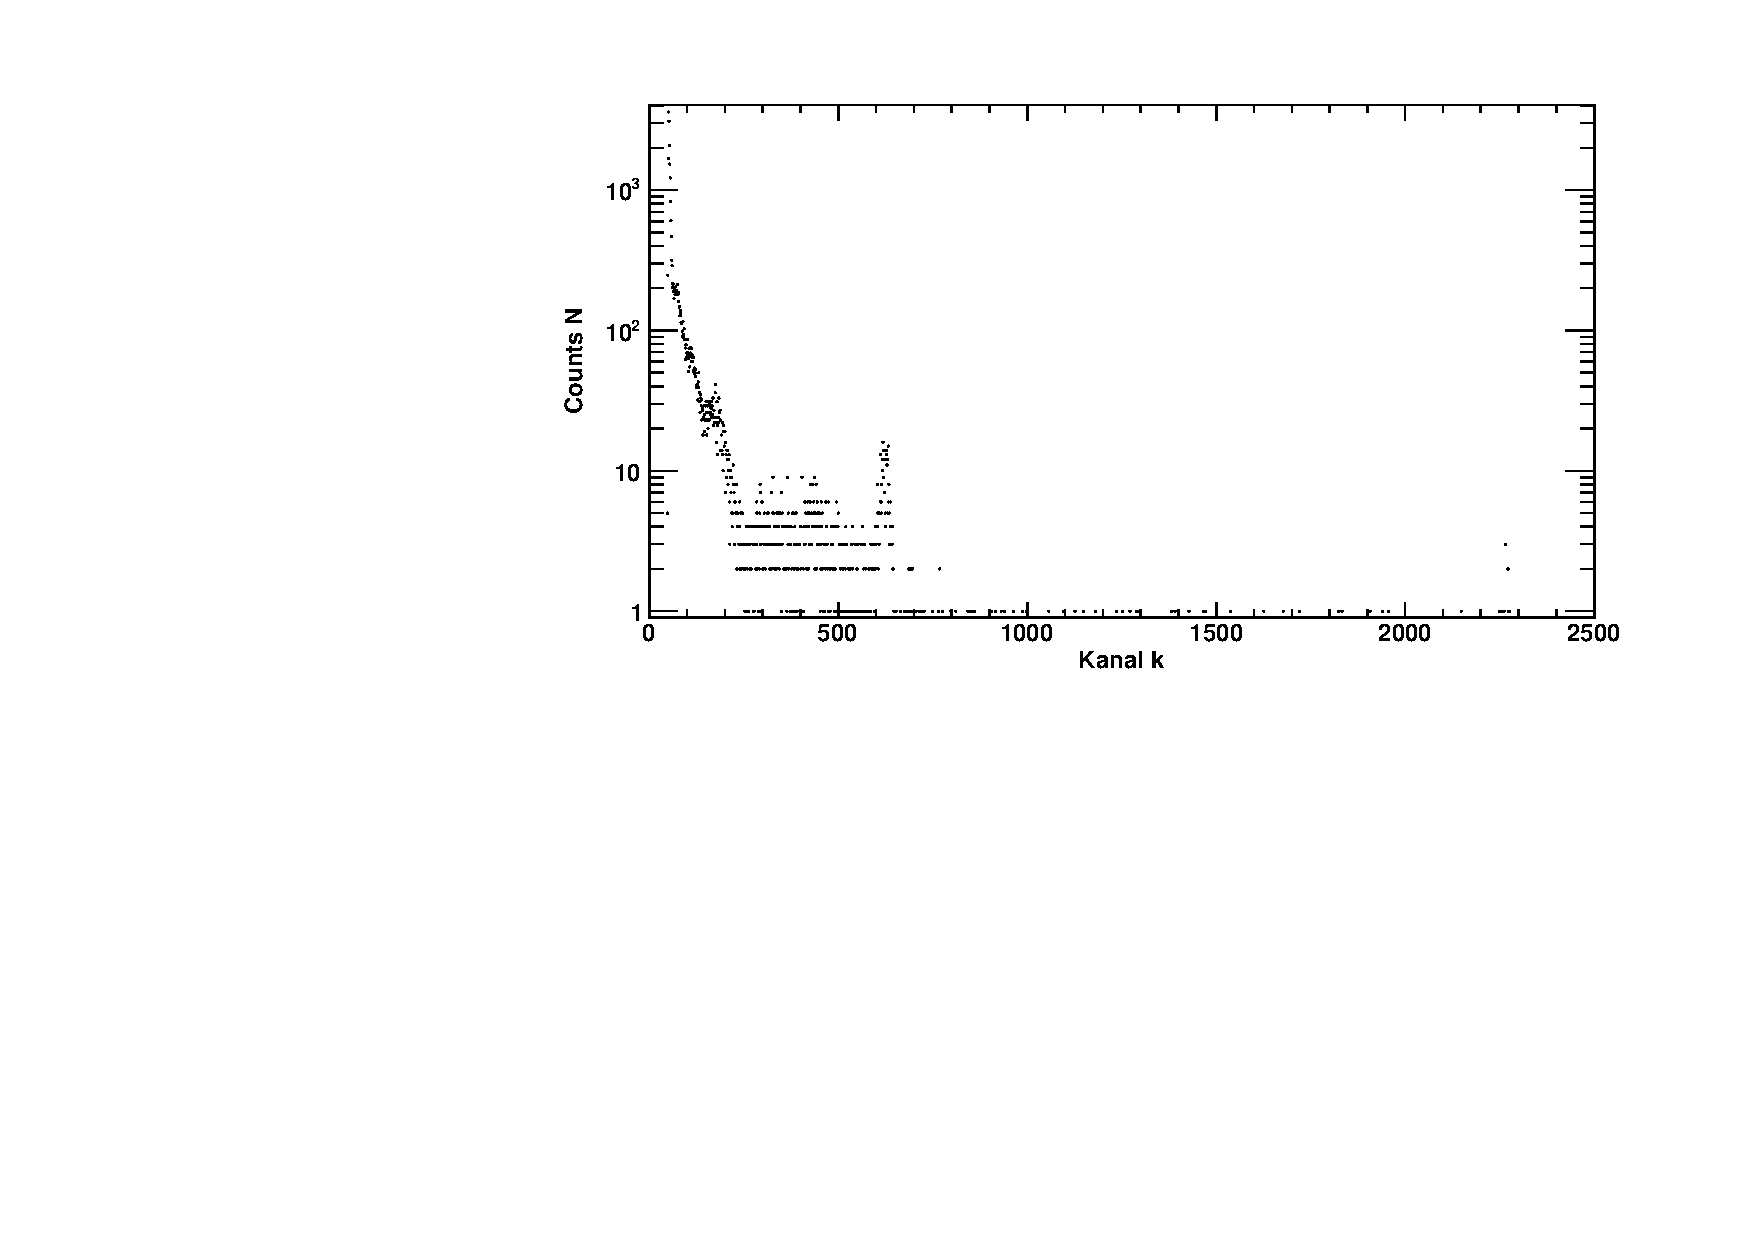
\includegraphics[width=\textwidth]{../img/part3/Co-Si_spectrum.pdf}
  \caption{Spektrum von \co, gemessen mit dem Si-Detektor.}
  \label{img:si:co:spektrum}
\end{center}
\end{figure}

\begin{figure}[H]
\begin{center}
  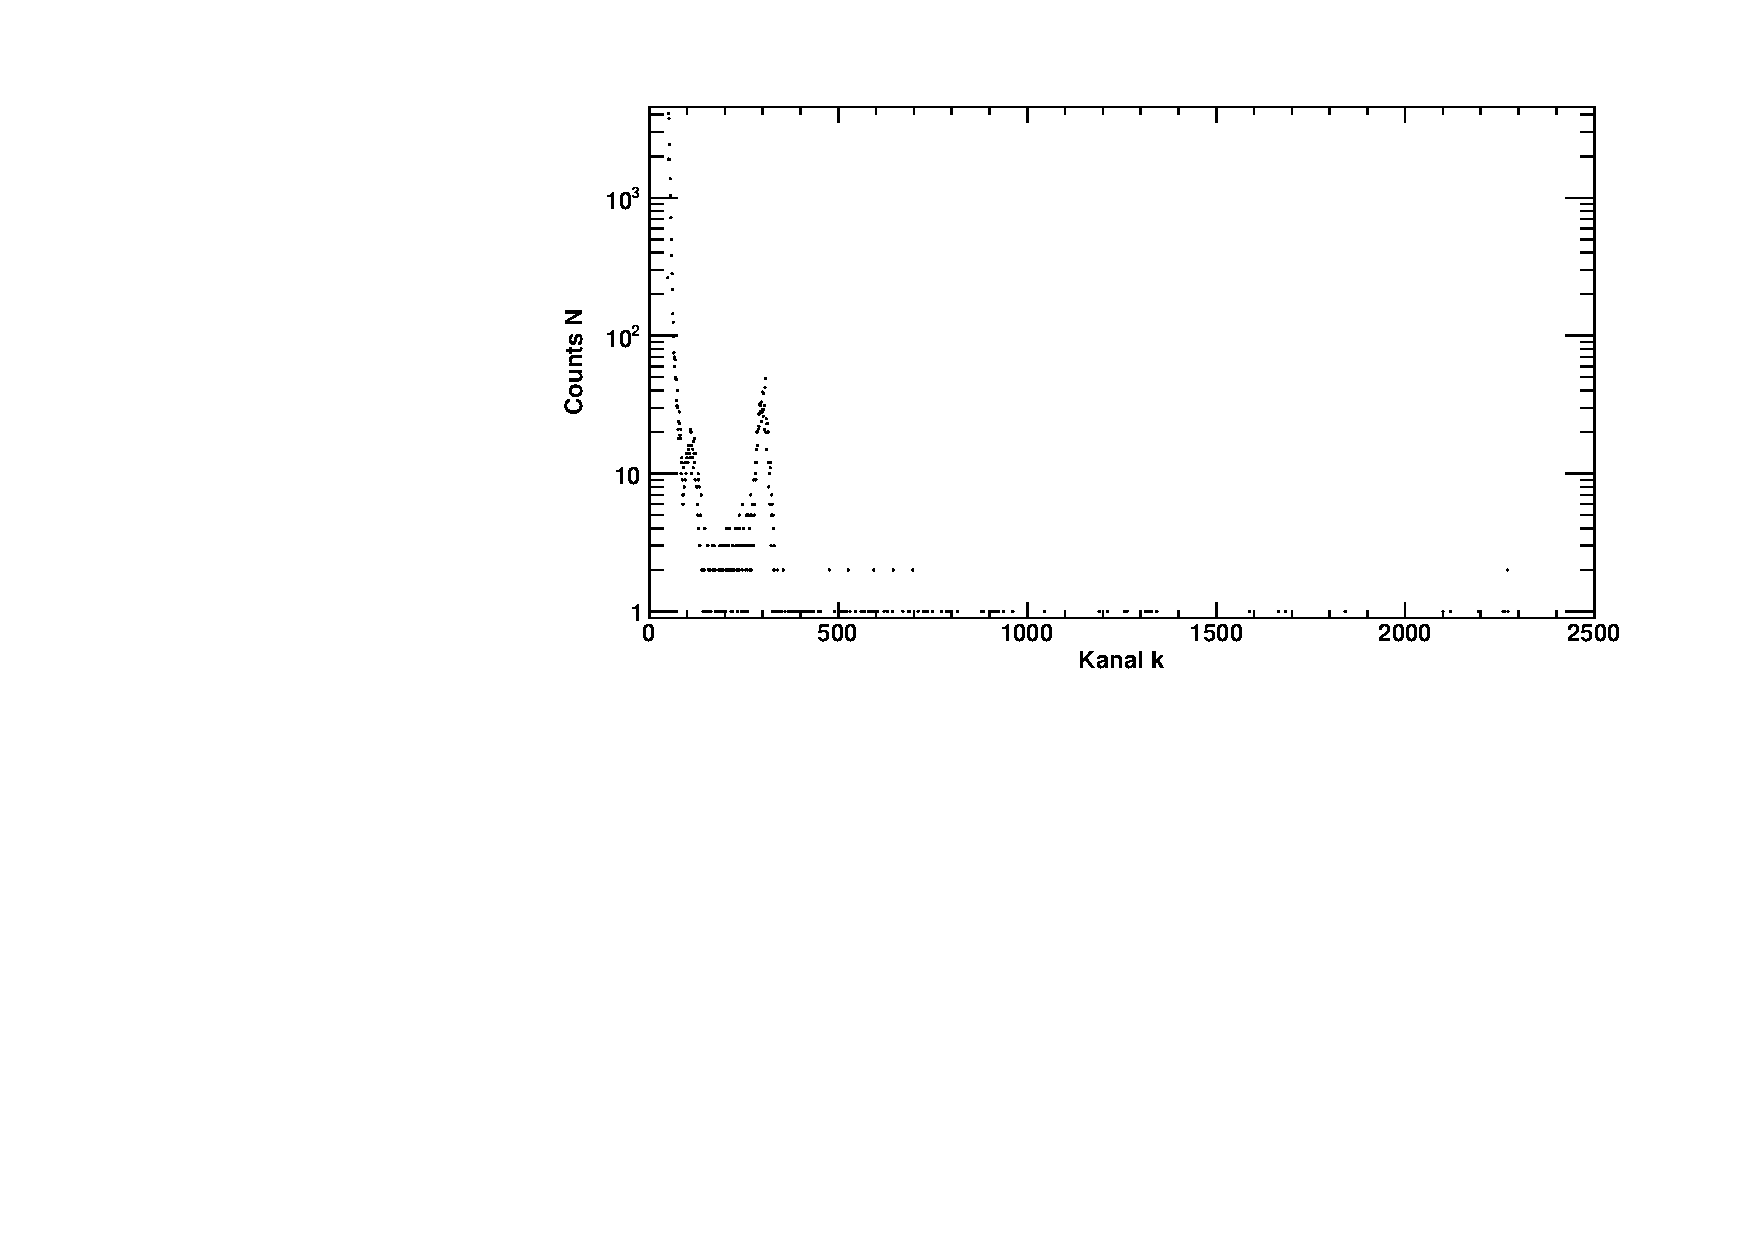
\includegraphics[width=\textwidth]{../img/part3/Am-Si_spectrum.pdf}
  \caption{Spektrum von \am, gemessen mit dem Si-Detektor.}
  \label{img:si:am:spektrum}
\end{center}
\end{figure}

\paragraph{Peaks}
Die Peaks werden wieder mit der normierten Gaußkurve (\autoref{eq:part3:normgauss}) gefittet 
(\autoref{img:am:si:peak0}, \autoref{img:co:si:peak0} und \autoref{img:co:si:peak1}). Jedoch hat der 136.47\,keV-Peak von \co eine zu kleine 
Anzahl von Counts, dass man noch gut eine Gaußkurve erkennen und anpassen kann. Im nächsten Abschnitt wird erklärt, wie man doch noch 
Informationen über die Lage und Ausdehnung des Peaks erhalten kann.
\begin{figure}[H]
\begin{center}
  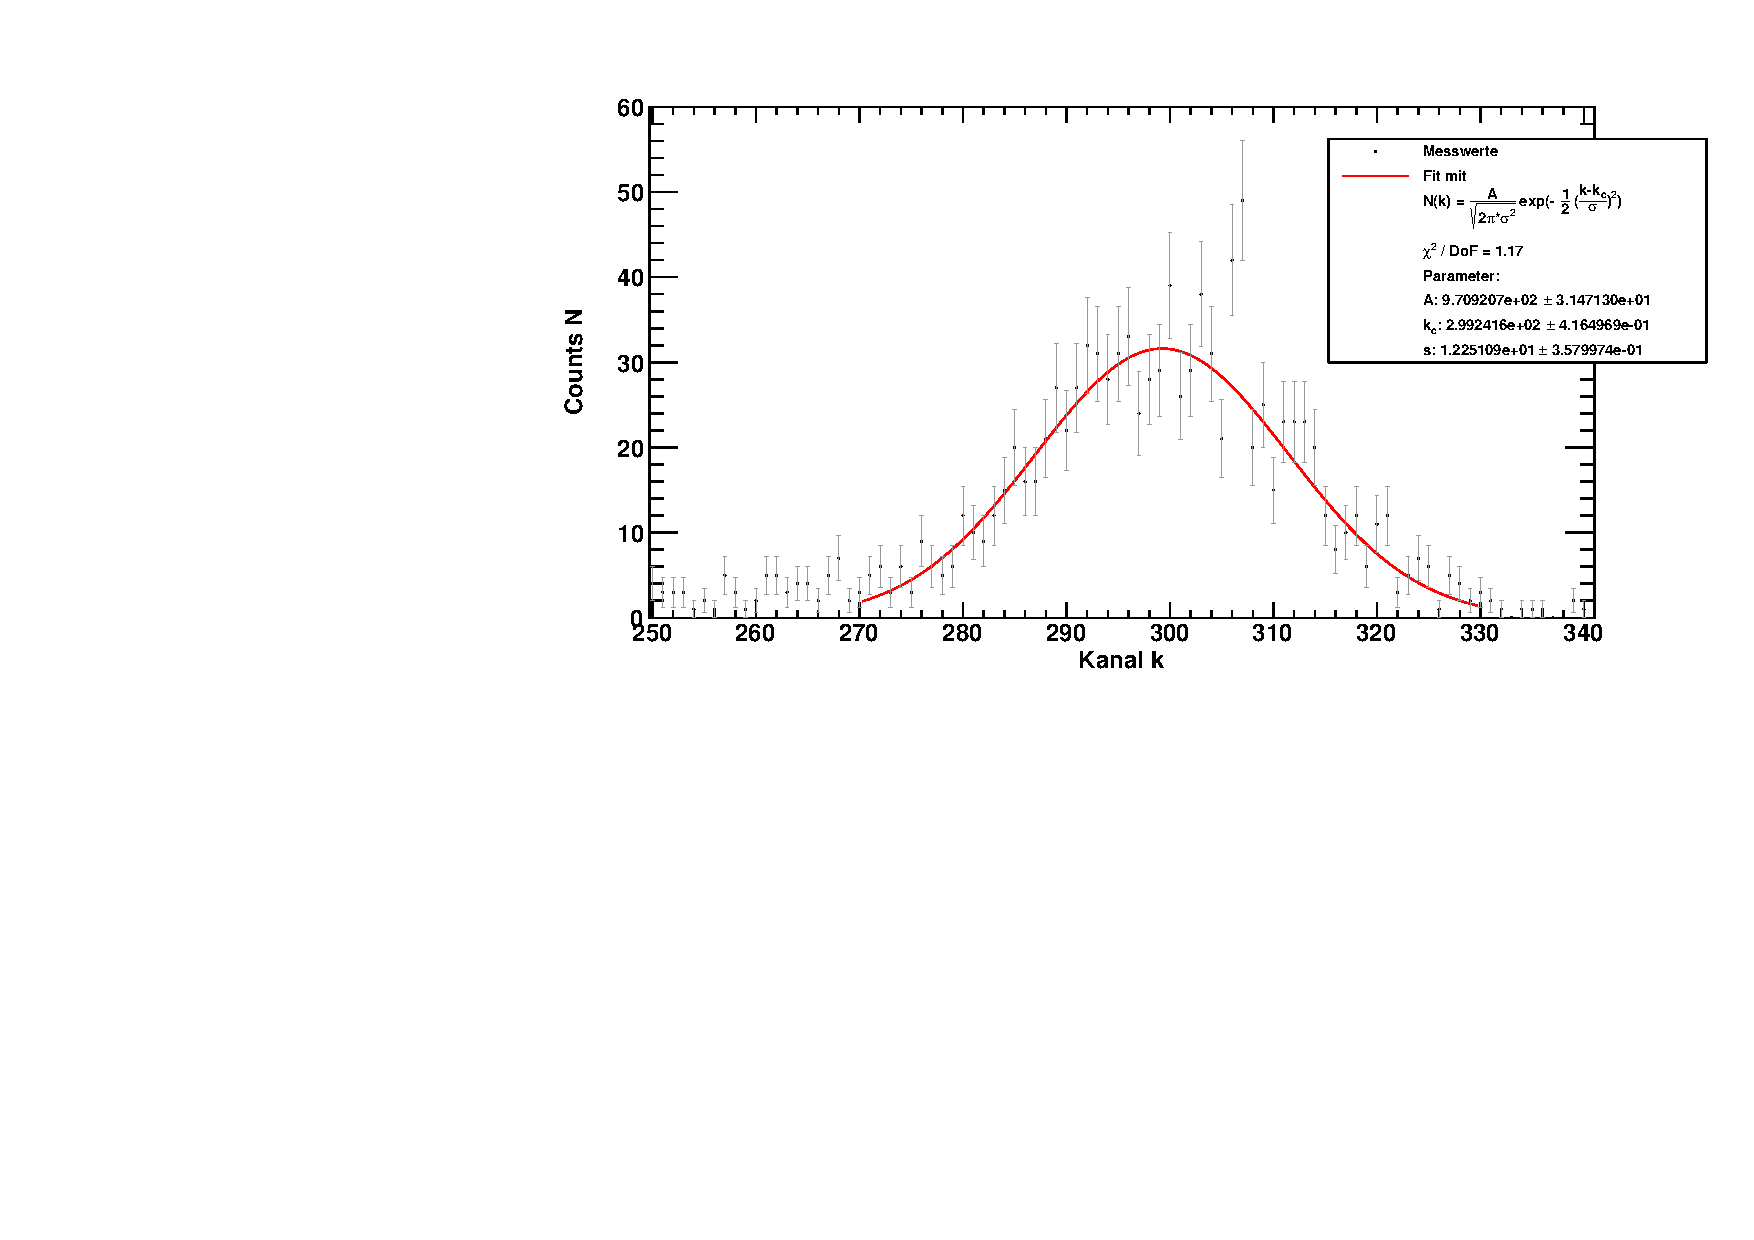
\includegraphics[width=\textwidth]{../img/part3/Am-Si_00.pdf}
  \caption{59.5\,keV-Peak von \am, gemessen mit dem Si-Detektor.}
  \label{img:am:si:peak0}
\end{center}
\end{figure}

\begin{figure}[H]
\begin{center}
  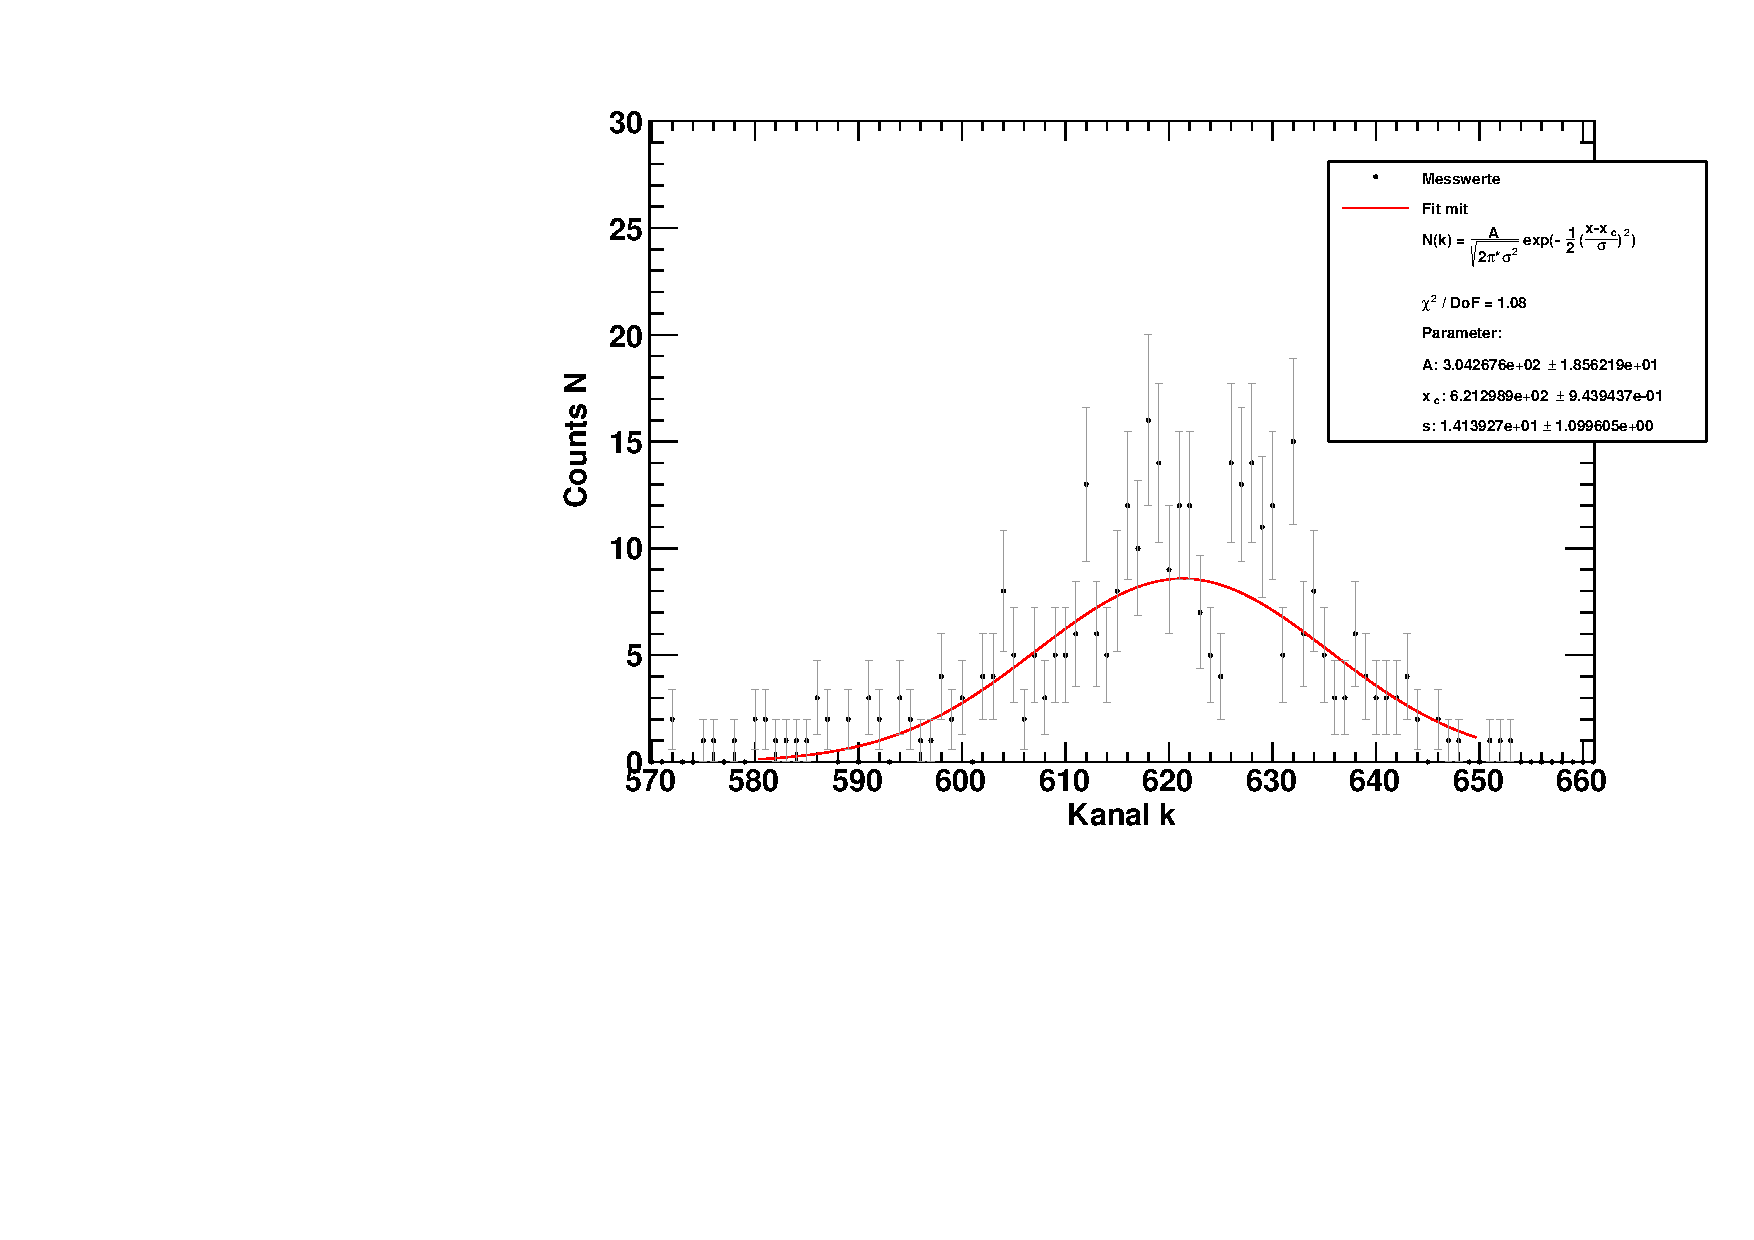
\includegraphics[width=\textwidth]{../img/part3/Co-Si_00.pdf}
  \caption{122.06\,keV-Peak von \co, gemessen mit dem Si-Detektor.}
  \label{img:co:si:peak0}
\end{center}
\end{figure}

\begin{figure}[H]
\begin{center}
  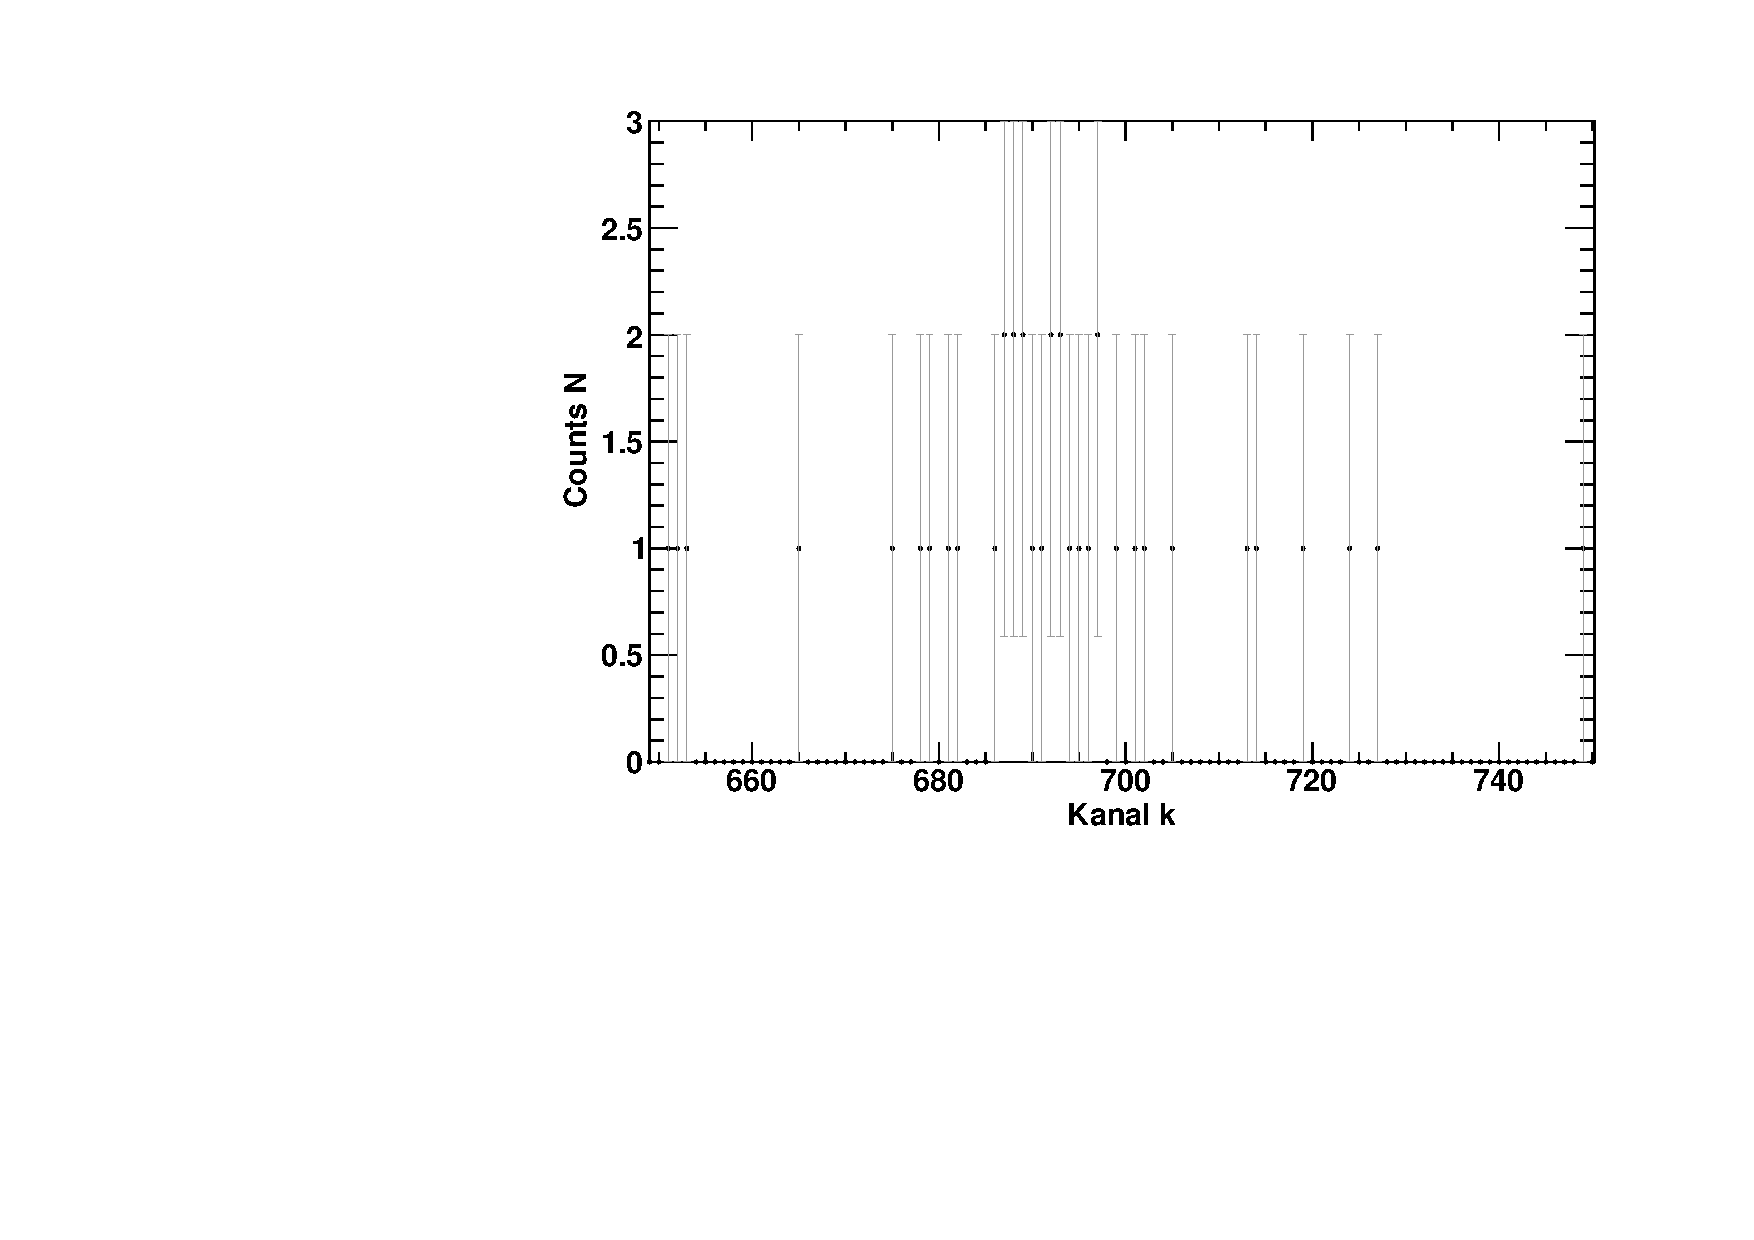
\includegraphics[width=\textwidth]{../img/part3/Co-Si_01.pdf}
  \caption{136.47\,keV-Peak von \co, gemessen mit dem Si-Detektor.}
  \label{img:co:si:peak1}
\end{center}
\end{figure}

\paragraph{Bestimmung des 136.47\,keV-Peak von \co}
Platzhalter

\begin{figure}[H]
\begin{center}
  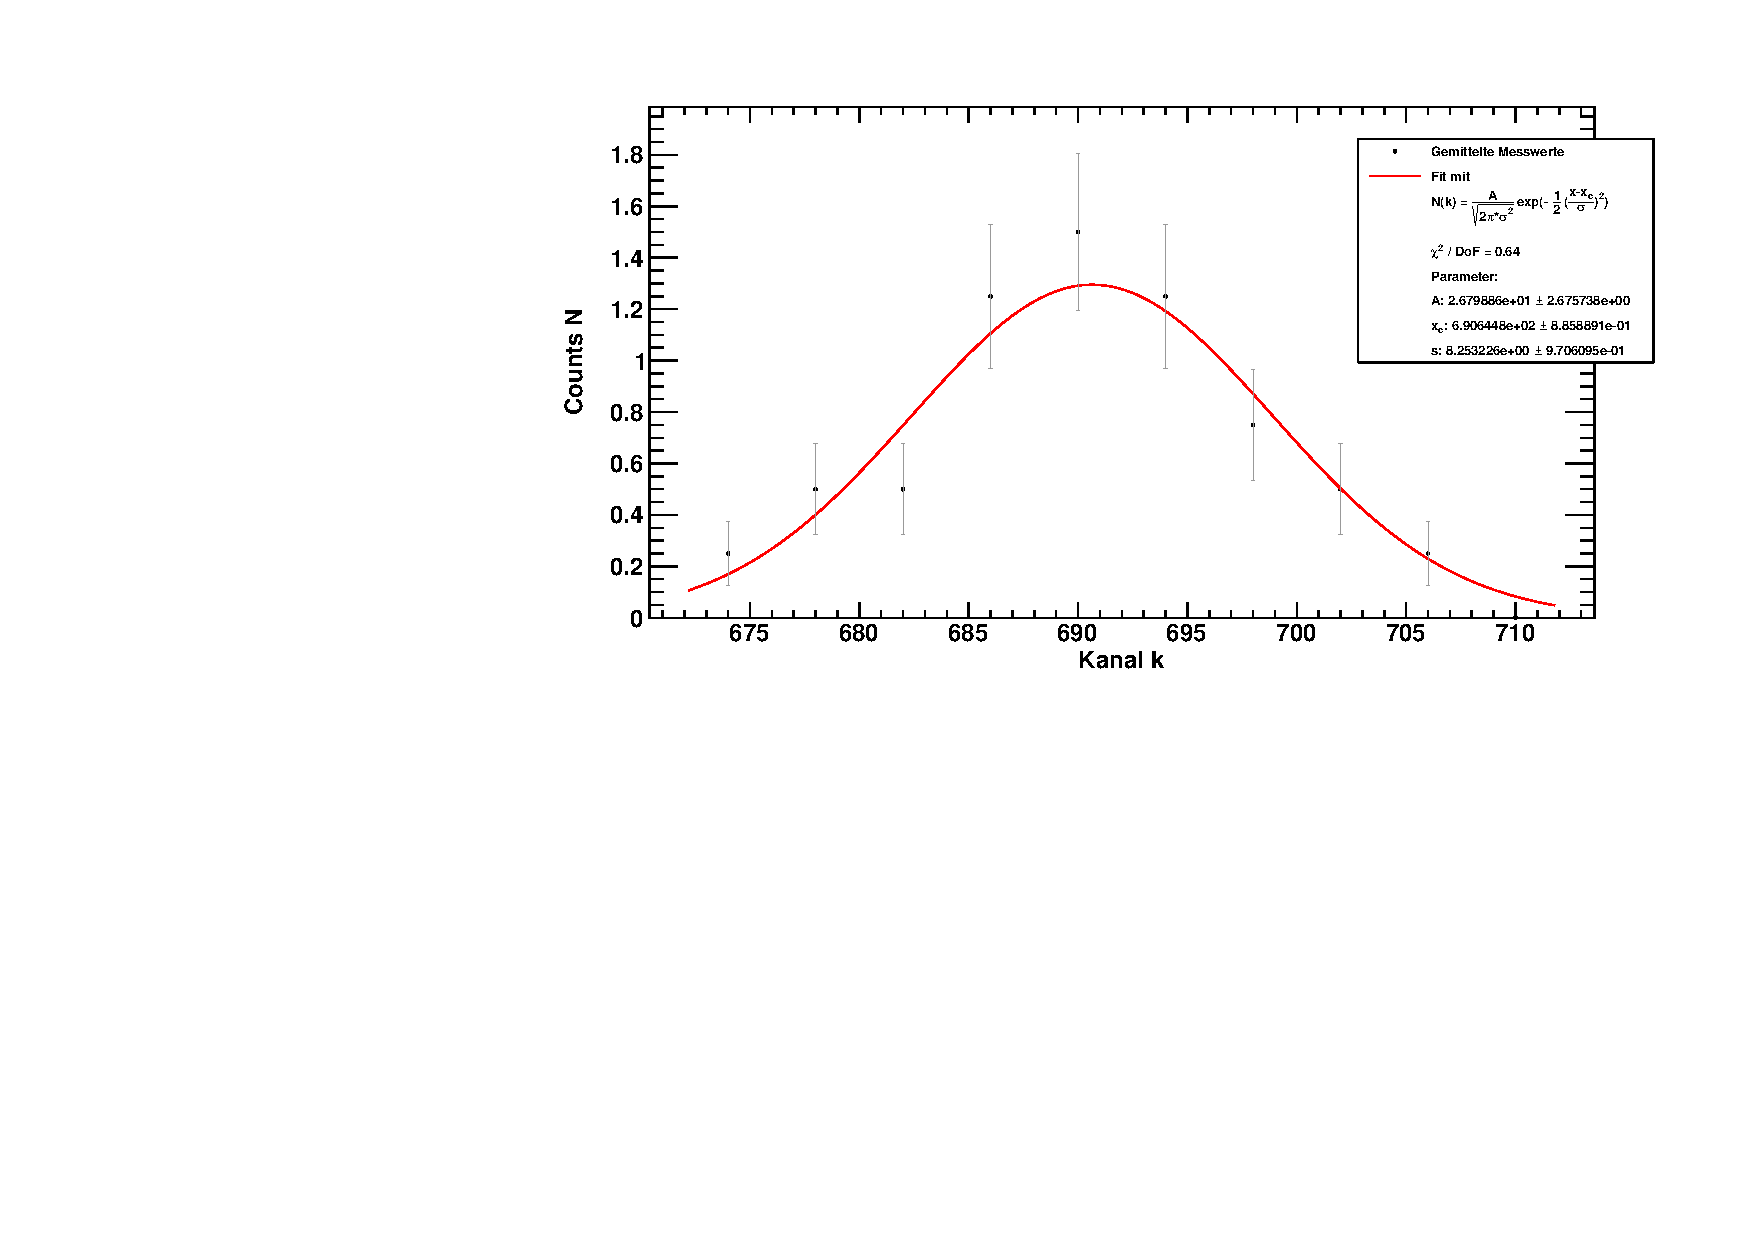
\includegraphics[width=\textwidth]{../img/part3/Co-Si_01_mergedbins.pdf}
  \caption{136.47\,keV-Peak von \co, gemessen mit dem Si-Detektor. Jeweils 5 Kanäle wurden zusammengefasst.}
  \label{img:co:si:peak1}
\end{center}
\end{figure}

\paragraph{Energieeichung}
Platzhalter

\begin{figure}[H]
\begin{center}
  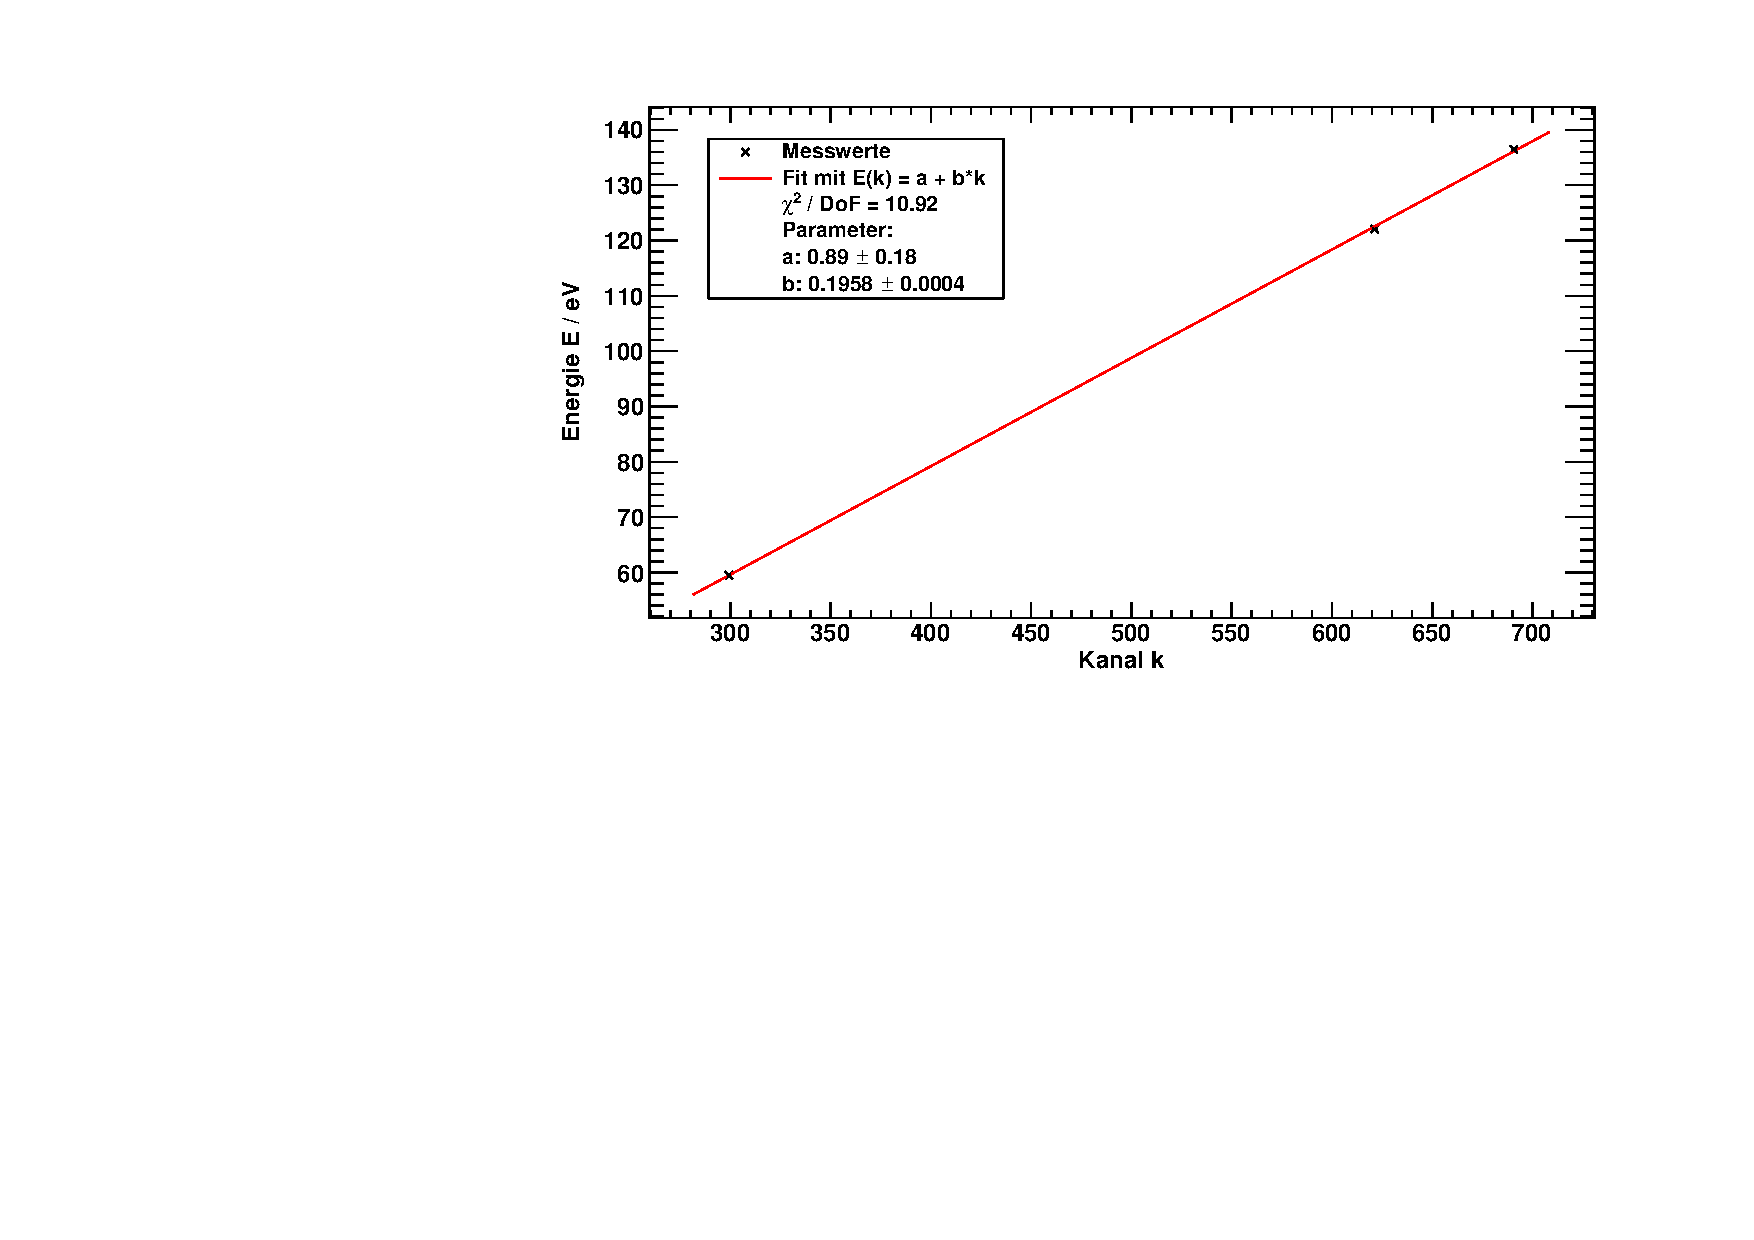
\includegraphics[width=\textwidth]{../img/part3/energygauge_Si.pdf}
  \caption{caption}
  \label{img:si:energygauge}
\end{center}
\end{figure}

\paragraph{Absorptionswahrscheinlichkeiten}

\paragraph{Relative Energieauflösung}

\subsubsection{Absorptionsverhältnisse}